\documentclass[12pt,a4paper]{article}
\usepackage[utf8]{inputenc}
\usepackage[brazil]{babel}
\usepackage{graphicx}
\usepackage{amssymb, amsfonts, amsmath}
\usepackage{float}
\usepackage{enumerate}
\usepackage[top=2.5cm, bottom=2.5cm, left=1.25cm, right=1.25cm]{geometry}

\begin{document}
\pagestyle{empty}

\begin{center}
  \begin{tabular}{ccc}
    \begin{tabular}{c}
      
\includegraphics[scale=0.25]{../../biblioteca/imagem/brasao-de-armas-brasil} \\
    \end{tabular} & 
    \begin{tabular}{c}
      Ministério da Educação \\
      Universidade Federal dos Vales do Jequitinhonha e Mucuri \\
      Faculdade de Ciências Sociais, Aplicadas e Exatas - FACSAE \\
      Departamento de Ciências Exatas - DCEX \\
      Disciplina: Cálculo Numérico \quad Semestre: 2024/1\\
      Prof. Dr. Luiz C. M. de Aquino\\
    \end{tabular} &
    \begin{tabular}{c}
      
\includegraphics[scale=0.25]{../../biblioteca/imagem/logo-ufvjm} \\
    \end{tabular}
  \end{tabular}
\end{center}

\begin{center}
  \textbf{Lista I}
\end{center}

\begin{enumerate}
  \item Utilize os conhecimentos de Cálculo para provar que os gráficos das
  funções definidas por $f(x) = \cos\left(x^2\right)$ e $g(x) = x^3$ possuem
  um único ponto de interseção. Em seguida, de alguma maneria utilize o Método
  da Bisseção para determinar de modo aproximado esse ponto (considere uma
  tolerância de $10^{-4}$).

  \item A cada passo no Método da Falsa Posição, escolhemos 
  $x_k = \dfrac{a_k|f(b_k)| + b_k|f(a_k)|}{|f(a_k)|+|f(b_k)|}$, sendo que no
  intervalo $[a_k;\,b_k]$ temos $f(a_k)f(b_k)<0$. Prove que esta escolha de
  $x_k$ coincide com a abscissa do ponto de interseção entre o eixo $x$ e a reta
  passando por $(a_k,\,f(a_k))$ e $(b_k,\,f(b_k))$.

  \item Suponha que o custo para produzir $x$ unidades de certo produto seja aproximadamente 
  dado por $C(x) = \dfrac{1}{2}x^{\frac{2}{3}} + 12x + 1000$. Se esse produto for vendido por
  R\$ 20,00 a unidade, então a partir de qual quantidade não haverá prejuízo? Observação: 
  use o método de Newton na solução.

  \item De uma chapa de alumínio, com dimensão de 30 cm $\times$ 20 cm, serão recortados quatro
  quadrados de lado medindo $x$ cm, como ilustra a figura abaixo. Em seguida, a chapa será dobrada
  de modo a formar uma caixa sem tampa. Determine o valor de $x$ no intervalo [0, 2] para o qual 
  o volume dessa caixa seja 100 cm$^3$. Observação: use o método de Newton na solução com tolerância
  de $10^{-4}$.
  
  \begin{figure}[h]
    \centering
    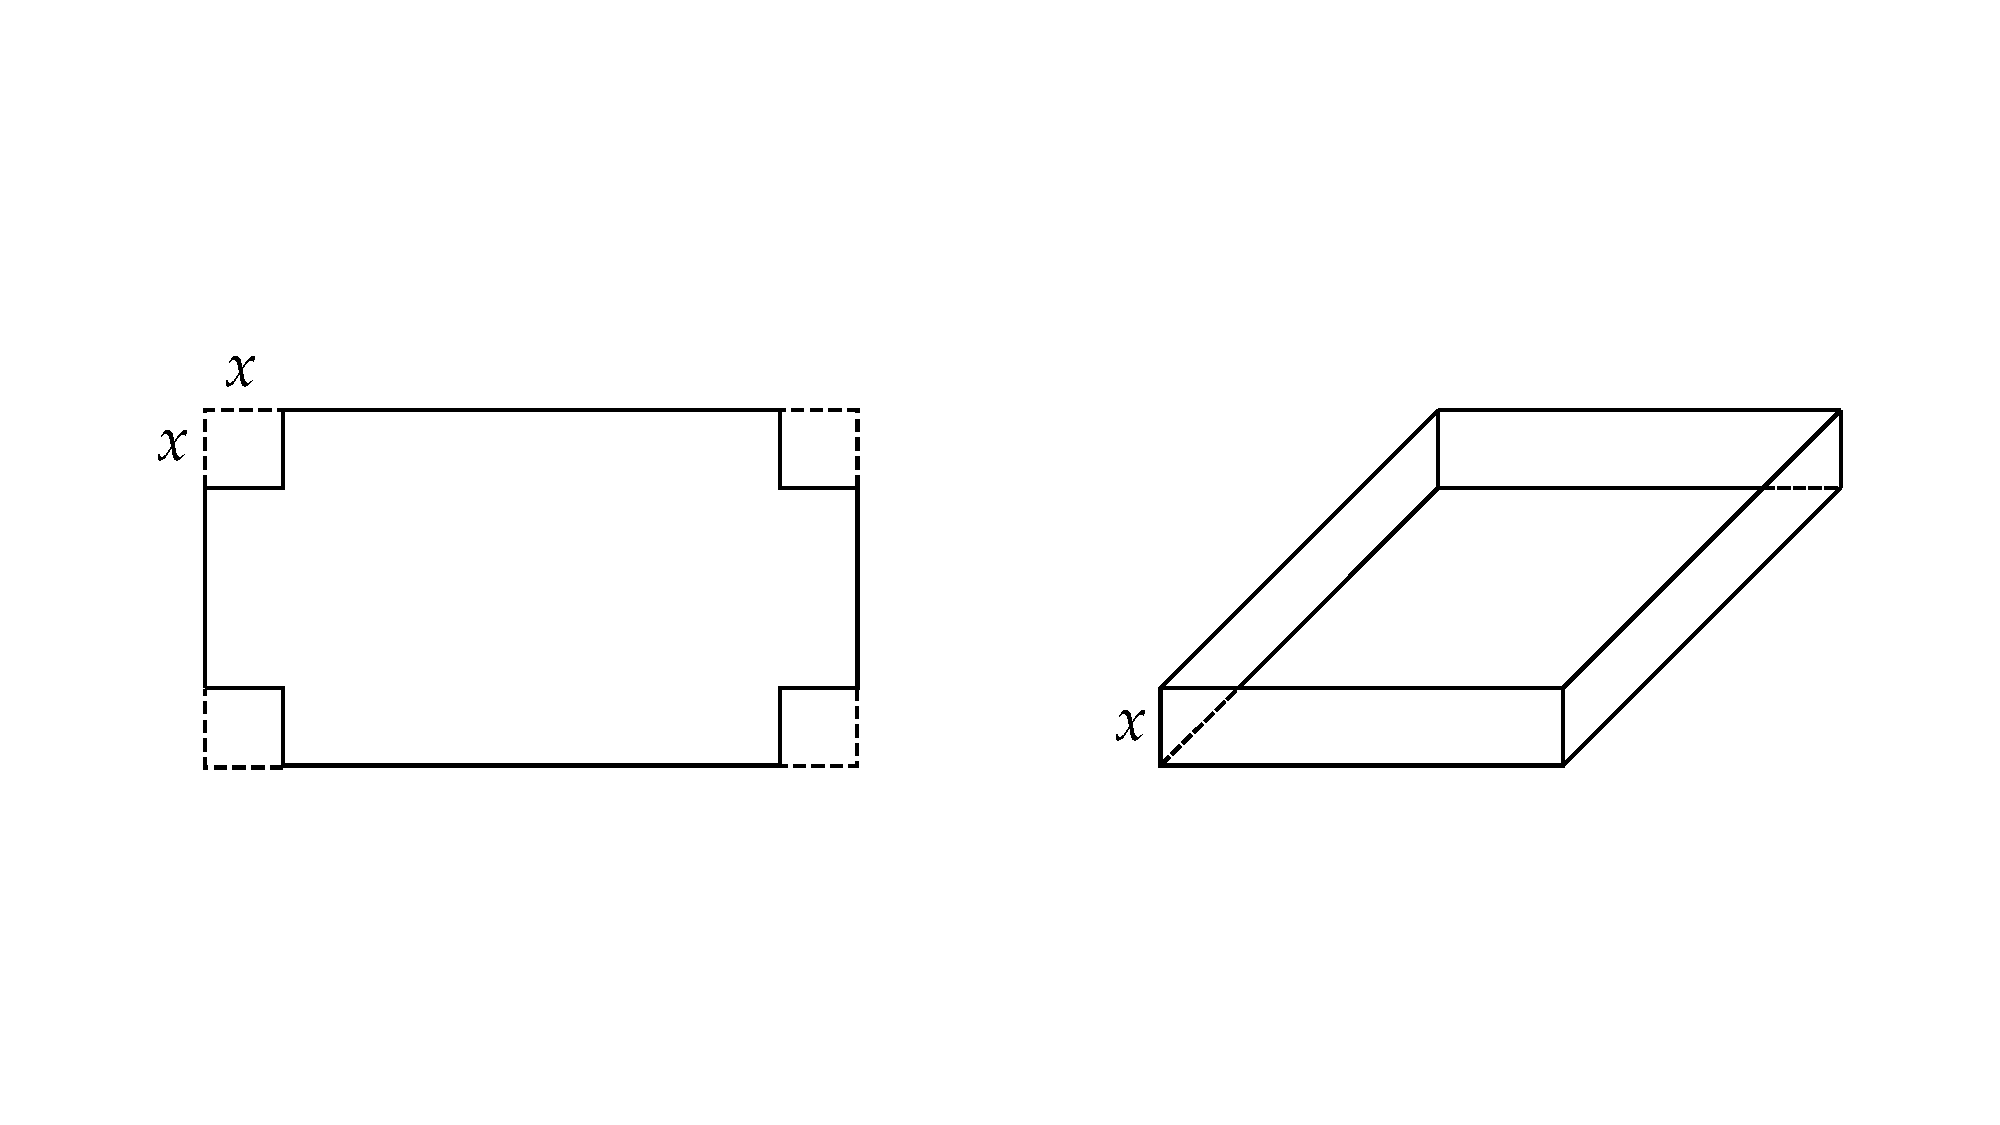
\includegraphics[scale=0.4]{imagem/caixa-retangular.pdf}
  \end{figure}

  \item Use o método de Newton para calcular o valor aproximado de $\sqrt[100]{100}$.
  Observação: use uma tolerância de $10^{-4}$.
     
\end{enumerate}

\begin{center}
  \textbf{Gabarito}
\end{center}
  \textbf{[1]} Sugestão: considerando $h(x) = f(x) - g(x)$, analise o valor de 
$h(0)h(1)$ e de $h'$ em $[0;\,1]$. Ponto de interseção aproximado:
$(0,889282226562501;\,0,703264730191224)$. 
  \textbf{[2]} Sugestão: determine a equação da reta que passa por $(a_k,\,f(a_k))$
  e $(b_k,\,f(b_k))$. Em seguida, calcule a abscissa do ponto de interseção entre esta
  reta e o eixo $x$.
  \textbf{[3]} A partir de 127 unidades. 
  \textbf{[4]} $x \approx 0,17153705$. 
  \textbf{[5]} $\sqrt[100]{100} \approx 1,04712855$. 
\end{document}